\documentclass[11pt,a4paper]{report}

% ================================================================
% Packages
% ================================================================
\usepackage{booktabs}
\usepackage[utf8]{inputenc}
\usepackage[T1]{fontenc}
\usepackage{lmodern}

\usepackage[margin=2.5cm]{geometry}
\makeatletter
\setlength{\@fptop}{0pt}
\setlength{\@fpsep}{12pt}
\setlength{\@fpbot}{0pt plus 1fil}
\makeatother
\usepackage{amsmath, amssymb}
\usepackage{siunitx}
\usepackage{graphicx}
\usepackage{pgf}
\usepackage{booktabs}
\usepackage{array}
\usepackage{float}
\usepackage{enumitem}
\usepackage{xcolor}
\usepackage{hyperref}
\usepackage{tocloft}
\usepackage{tabularx}
\usepackage{comment}
% ================================================================
% Hyperref
% ================================================================

\hypersetup{
	colorlinks=true,
	linkcolor=black,
	urlcolor=blue,
	citecolor=black
}

% ================================================================
% Table of Contents Style
% ================================================================

\renewcommand{\contentsname}{Contents}

\renewcommand{\cfttoctitlefont}{\normalfont\Huge}
\renewcommand{\cftaftertoctitle}{\vskip 2em}

\renewcommand{\cftchapfont}{\bfseries}
\renewcommand{\cftchappagefont}{\bfseries}

\setlength{\cftbeforechapskip}{0.5em}
\setlength{\cftbeforesecskip}{0.2em}

% ================================================================
% Document
% ================================================================

\begin{document}
	
	% ================================================================
	% TITLE PAGE
	% ================================================================
	
	\begin{titlepage}
		
		\vspace*{2.2cm}
		
		% ------------------------------------------------
		% Upper thin line
		% ------------------------------------------------
		
		\noindent\rule{\textwidth}{0.7pt}
		
		\vspace{0.35cm}
		
		% ------------------------------------------------
		% Title
		% ------------------------------------------------
		
		\begin{center}
			
			{\LARGE\bfseries
				From Coins to Combat: A Curriculum-Trained PPO Agent for Bomberman
			}
			
		\end{center}
		
		\vspace{0.35cm}
		
		% ------------------------------------------------
		% Lower thick line
		% ------------------------------------------------
		
		\noindent\rule{\textwidth}{4pt}
		
		\vspace{1.8cm}
		
		% ------------------------------------------------
		% Authors and Course Information
		% ------------------------------------------------
		
		\noindent
		\begin{minipage}[t]{0.47\textwidth}
			
			\textit{Author:}
			
			\vspace{0.15cm}
			
			\textbf{Qin Yan}\\
			Individual part of a group project
			
		\end{minipage}
		\hfill
		\begin{minipage}[t]{0.47\textwidth}
			
			\raggedleft
			
			\textit{Machine Learning Essentials}\\
			Summer Semester 2026\\
			Heidelberg University
			
		\end{minipage}
		
		\vfill
		
		% ------------------------------------------------
		% Repository
		% ------------------------------------------------
		
		\begin{center}
			
			\textbf{Code Repository:}
			
			\vspace{0.4cm}
			
			\url{https://github.com/QinYan03/bomberman-rl-rhine}
			
		\end{center}
		
		\vfill
		
		% ------------------------------------------------
		% Date
		% ------------------------------------------------
		
		\begin{center}
			September 28, 2026
		\end{center}
		
		\vspace{1cm}
		
	\end{titlepage}
	
	\begin{abstract}
		This report presents RHINE, a reinforcement learning agent for a simplified multi-player version of Bomberman, developed as the author's individual part of a group project in the course Machine Learning Essentials at Heidelberg University. RHINE is a proximal policy optimization agent with an actor-critic multilayer perceptron that acts on 31 engineered features. A rule-based mask removes illegal actions and actions that lead to a known, unavoidable death, and the policy chooses among the remaining ones. The agent was trained from scratch through a four-task curriculum, from coin collection on an empty board to the full game against three rule-based opponents. In 100 games per training seed against three \texttt{rule\_based\_agent}s, it scored 6.33 points per game on average, against 5.04 for the best opponent in each game, and finished alone in first place in 53\% of games. Most of its remaining deaths arise from same-step contests for a tile, whose outcome the agent cannot control.
	\end{abstract}
	% ================================================================
	% TABLE OF CONTENTS
	% ================================================================
	
	\clearpage
	
	\tableofcontents
	
	\clearpage
	
	\graphicspath{{figures/}}
	
	% ================================================================
	% INTRODUCTION
	% ================================================================
	
	\chapter{Introduction}
	\label{chap:introduction}
	
	The game is played by four agents on a 17$\times$17 board of walls, crates and free tiles. In every step, each agent chooses one of six actions: a move in one of the four directions, WAIT or BOMB. A bomb explodes 4 steps after it is placed and destroys crates and agents up to 3 tiles away in each straight direction, unless a wall blocks the blast. Destroyed crates may reveal coins. Collecting a coin scores one point and killing an opponent scores five. A round lasts at most 400 steps.
	
	The agent has to decide within 0.5~s per step on a single CPU thread, and no training takes place during play. It is evaluated against the framework's scripted \texttt{rule\_based\_agent} and finally in a tournament against the agents of other groups, whose behaviour is unknown in advance.
	
	The course structures the problem into four tasks of increasing difficulty: collecting coins on a board without crates or opponents (Task~1), clearing crates with bombs without opponents (Task~2), playing against passive and coin-collecting opponents (Task~3), and playing the full game against three \texttt{rule\_based\_agent}s (Task~4). RHINE was developed independently by the author within a three-person group, in which the other members developed separate agents. This report covers RHINE only. Chapter~\ref{chap:methods} describes the final design, Chapter~\ref{chap:training} the training procedure, Chapter~\ref{chap:results} the experiments that led to the final design together with the results, and Chapter~\ref{chap:conclusion} the conclusions.
	
	% ================================================================
	% 4. METHODS
	% ================================================================
	
	\chapter{Methods}
	\label{chap:methods}
	\label{sec:rhine_methods}
	
	\section{Overview}
	\label{subsec:rhine_methods_overview}
	
	RHINE is a proximal policy optimization (PPO) agent~\cite{schulman2017ppo} with an actor-critic multilayer perceptron that acts on a compact vector of engineered features. Each game state is first reduced to model-independent semantic quantities (breadth-first-search distances, blast coverage, time-dependent danger), from which a 31-dimensional feature vector is built. A rule-based action mask removes actions that are illegal or lead to a known, unavoidable death; the policy then chooses among the remaining actions. The division of labour is deliberate: the mask decides what must never be done, the features supply the information needed for a decision, the reward expresses which outcomes are preferred, and the network learns the relative long-term value of the remaining legal actions. No feature encodes a recommended action. The features describe distances, directions and risks, and the choice is learned.
	
	The design was built up over the four tasks. The following subsections describe the final form and state in which task each component was introduced, while the development history and the variants that were discarded are reported in Chapters~\ref{sec:rhine_training} and~\ref{sec:rhine_results}.
	
	\section{State representation}
	\label{subsec:rhine_features}
	
	Table~\ref{tab:rhine_features} lists the 31 features. All distances are shortest-path lengths computed by breadth-first search over passable tiles, rather than Manhattan distances, because walls and crates make the two differ substantially. When several targets or first steps are equally short, all corresponding direction flags are set, so the network rather than an arbitrary tie-break decides between them. Distances are divided by 16 and clipped at 1. Compared with an initial normalization by 32, this spreads out the short distances that matter most, while distances of 16 or more are rare.
	
	\begin{table}[htbp]
		\centering
		\small
		\begin{tabular}{llcl}
			\toprule
			Group & Features & Dim. & Task \\
			\midrule
			Movement & legality of the four moves & 4 & 1 \\
			Coins & reachable coin exists; distance; first-step directions & 6 & 1 \\
			Bombing & bomb available; bombing target exists; distance; & 8 & 2 \\
			& first-step directions; crates destroyed at the target & & \\
			Danger & current tile in danger; time to the nearest threat & 2 & 2 \\
			Competition & an opponent is at least as close to the target coin & 1 & 3 \\
			Kill target & a tile whose blast covers an opponent exists; distance; & 7 & 3 \\
			& first-step directions; escape difficulty of the covered opponent & & \\
			Opponent proximity & distance to the nearest opponent; opponents within & 3 & 4 \\
			& three steps; tiles reachable within six steps & & \\
			\bottomrule
		\end{tabular}
		\caption{The 31 input features and the task in which each group was introduced.}
		\label{tab:rhine_features}
	\end{table}
	
	The bombing target is the reachable tile that maximizes $c/(d+1)$, where $c$ is the number of crates a bomb there would destroy and $d$ is the travel distance, so that a nearby tile destroying few crates can be preferred to a distant one destroying many. The kill-target group is built in the same way: among the tiles from which a bomb would cover an opponent's current position, it points to the one that maximizes $e/(d+1)$ and reports $e$, the escape difficulty of the covered opponent, a score in $[0,1]$ based on how few escape routes the opponent has before detonation. When several opponents are covered, $e$ is their maximum, because a sum would let several unlikely kills outweigh a near-certain one. Opponents carry no type label, since the agents in the final tournament are unknown. Thus, the policy must infer an opponent's threat from its behaviour. The feature vector is purely Markovian: it contains no history of past positions or actions.
	
	
	\section{Action masking and evaluation-time oscillation breaker}
	\label{subsec:rhine_mask}
	
	The action mask is applied to the policy's logits during both training and evaluation, following the standard practice for invalid-action masking in policy gradient methods~\cite{huang2022masking}. It removes moves into walls, crates, bombs or other agents, as well as moves onto a tile that a known bomb will hit before the agent can leave it. BOMB is removed whenever no escape route exists after placing the bomb. Opponents' current positions are treated as temporary obstacles, recomputed at every step, and the agent does not predict opponents' future moves. The escape check was strengthened in Task 3 after opponents were found to block escape routes. A tile $t$ that the agent reaches $k$ steps after placing the bomb conflicts with opponent $j$ if $d_j(t) \le k$, where $d_j(t)$ is the opponent's current shortest-path distance to $t$. If $N$ distinct opponents cause conflicts, at least $\min(N+1, 4)$ escape routes that differ at every conflicting tile are required, and otherwise BOMB is masked. While in danger with several legal moves, the agent additionally avoids moves onto tiles that an opponent could reach on the next step, unless no other move remains. 
	
	At evaluation time only, an oscillation breaker is added on top of this mask. When the agent has been confined to at most two tiles over the last seven steps and a move other than returning is legal, the move back to the previous tile is masked. Dead ends are therefore left untouched, and the intervention is limited to six consecutive steps. The breaker was introduced in Task 2 and extended in Task 3 to recognize side branches. It changes behaviour without changing the network, so its effect is reported separately from learned improvements.
	
	\section{Reward design}
	\label{subsec:rhine_reward}
	
	Table~\ref{tab:rhine_reward} lists the final reward terms. Coins and kills are rewarded in a 1:3 ratio instead of the game's 1:5 scoring ratio. In a short Task 3 comparison, both $+3$ and $+5$ trained stably, but $+5$ gave a slightly higher value loss and lower explained variance, so $+3$ was kept. The penalty for being killed by an opponent was set symmetrically to $-3$ and not tested separately. All evaluations use the game's actual score, never the training reward.
	
	\begin{table}[htbp]
		\centering
		\small
		\begin{tabular}{lrl}
			\toprule
			Term & Value & Task \\
			\midrule
			Coin collected & $+1.0$ & 1 \\
			Step cost & $-0.01$ & 1 \\
			Crate destroyed (per crate) & $+0.1$ & 2 \\
			Progress towards the current target (per step of distance) & $0.10$ & 2 \\
			Confinement to $\le 2$ tiles over the last four steps with a bomb available (per step) & $-0.05$ & 2 \\
			Self-kill & $-2.0$ & 2, raised in 3 \\
			Opponent killed & $+3.0$ & 3 \\
			Killed by an opponent & $-3.0$ & 3 \\
			Bomb covering neither a crate nor an opponent & $-0.2$ & 3 \\
			\bottomrule
		\end{tabular}
		\caption{Final training reward terms and the task in which each was introduced.}
		\label{tab:rhine_reward}
	\end{table}
	
	The progress term is inspired by potential-based shaping~\cite{ng1999shaping}: its potential is the negative distance to the current target, which is the nearest reachable coin if one exists and the best bombing tile otherwise. Because the term is skipped on steps where the target changes, it is not strictly potential-based, and no policy-invariance guarantee is claimed. The confinement penalty depends on recent positions and targets the oscillation observed in Task 2 (Section~\ref{subsec:rhine_results_task2}), and the wasteful-bomb penalty depends on the chosen action, so neither is a function of the state alone.
	
	\section{Learning algorithm and network}
	\label{subsec:rhine_ppo}
	
	The actor and critic share a two-layer trunk of 64 tanh units each, followed by a linear policy head over the six actions and a linear value head. Training uses the clipped PPO objective with generalized advantage estimation~\cite{schulman2017ppo,schulman2016gae}, normalized advantages and the Adam optimizer. From Task 2 onwards, the value loss is computed on returns and value predictions normalized by a running mean and standard deviation of the returns. This keeps the value loss bounded and prevents it from dominating the entropy bonus. The hyperparameters are listed in Table~\ref{tab:rhine_hyperparameters}.
	
	\section{Evaluation protocol and metrics}
	\label{subsec:rhine_eval_protocol_metrics}
	
	Unless stated otherwise, every final evaluation uses a deterministic policy (the most probable action after masking) and 100 games with a fixed evaluation seed (1000, cross-checked with 2000 where stated). From Task 3 onwards, each configuration is trained with three independent training seeds and reported as mean~$\pm$~sample standard deviation across seeds, since single training runs of deep reinforcement learning agents can differ considerably~\cite{henderson2018matters}. During training, the policy was evaluated periodically, and the checkpoint used for the final evaluation was chosen as summarized in Table~\ref{tab:rhine_eval_settings}. These settings were refined over the course of the project. From Task 3 onwards, the checkpoint was selected among the five best periodic evaluations by score, discarding those whose self-kill rate or oscillation fraction (from Stage D onwards also killed-by-opponent rate) clearly exceeded the median over that seed's evaluations. From Stage D onwards, periodic evaluations used a separate evaluation seed, so that checkpoint selection and final evaluation are independent. Selection scores are not reported as results.
	
	\begin{table}[htbp]
		\centering
		\small
		\begin{tabular}{lll}
			\toprule
			Task & Periodic evaluation & Checkpoint used \\
			\midrule
			1 & 15 games every 50 rounds, seed 1000 & end of training \\
			2 & 15 games every 50 rounds, seed 1000 & snapshot screening (Section~\ref{subsec:rhine_training_task2}) \\
			3, Stages A--C & 50 games every 50 rounds, seed 1000 & best of five by score, filtered \\
			3, Stage D & 50 games every 100 rounds, seed 3000 & best of five by score, filtered \\
			4 & 50 games every 100 rounds, seed 3000 & best of five by score, filtered \\
			\bottomrule
		\end{tabular}
		\caption{Periodic evaluation during training and checkpoint selection in each task.}
		\label{tab:rhine_eval_settings}
	\end{table}
	
	The metrics are defined in Table~\ref{tab:rhine_metrics}. Against opponents, the final score of every agent is also recorded, to report RHINE's placement among the four agents.
	
	\begin{table}[htbp]
		\centering
		\small
		\begin{tabular}{lp{9cm}}
			\toprule
			Metric & Definition \\
			\midrule
			Score & Actual game score: one point per coin, five per kill \\
			Completion rate & Fraction of games in which all coins are collected by any agent \\
			Steps to completion & Mean length of completed games (Task~1 only, where a game ends with the last coin) \\
			Oscillation fraction & Fraction of games with at least ten consecutive moves alternating between two opposite directions \\
			Self-kill/ killed-by-opponent rate & Fraction of games in which RHINE dies from its own / an opponent's bomb \\
			Illegal actions & Moves into walls, crates, bombs or occupied tiles chosen by the agent (total over all games) \\
			Also reported & Steps per coin, wait fraction, crates destroyed, opponent kills \\
			\bottomrule
		\end{tabular}
		\caption{Evaluation metrics. Unless stated otherwise, metrics are means per game.}
		\label{tab:rhine_metrics}
	\end{table}
	
	The variants compared are:
	\begin{itemize}[noitemsep]
		\item \textbf{Task~1:} three reward configurations.
		\item \textbf{Task~2:} target-progress shaping, anti-oscillation mechanisms, training-stability measures and bombing-target selection.
		\item \textbf{Task~3:} a four-stage opponent curriculum and changes to the opponent feature groups.
		\item \textbf{Task~4:} the oscillation breaker, a deadlock bombing rule, and the Stage D agent as a baseline.
	\end{itemize}
	
	All results in this chapter and the following ones were obtained with the framework's per-step thinking-time limit disabled, so that occasional delays caused by concurrent load on the evaluation machine cannot force WAIT actions and distort the policy's measured behaviour. From Task 3 Stage D onwards, the opponents' random number generators were reseeded at the start of every game from the evaluation seed and the game index, and the Stage D baseline and all Task 4 evaluations were rerun with this setting, so that they are exactly reproducible. Any anomaly in the results could therefore be replayed and traced to its underlying pattern, against which a targeted change to the design was then developed. To confirm that the final agent stays within the 500~ms limit, its thinking time was measured separately in 20 games against three \texttt{rule\_based\_agent}s: the mean \texttt{act()} time was 15.8~ms and the maximum 125.2~ms, roughly 155~ms when scaled to the tournament processor by PassMark ratings. Across this and a second run of the same length, the framework recorded 3 overruns in 11{,}010 calls, each of about 1.4~s. These pauses far exceed the processor time measured for any \texttt{act()} call and therefore arose outside the policy computation, but their cause was not investigated.
	
	% ================================================================
	% 5. TRAINING
	% ================================================================
	
	\chapter{Training}
	\label{chap:training}
	\label{sec:rhine_training}
	
	\section{Overview}
	\label{subsec:rhine_training_overview}
	
	Training followed a curriculum~\cite{bengio2009curriculum} that mirrors the four tasks, with one new difficulty at a time: navigation on an empty board (Task 1), crates and bombs without opponents (Task 2), passive and then coin-collecting opponents (Task 3), and finally the full-strength \texttt{rule\_based\_agent} (Task 4). Weights were not transferred between tasks or between the stages of Task 3: every configuration was trained from a random initialization, so that habits learned in an easier setting could not carry over and each result could be attributed to that stage's own feature and reward designs. Full weight transfer would in any case have been impossible, since the feature vector changed every task. All training runs disabled the thinking-time limit and, unless stated otherwise, used the hyperparameters in Table~\ref{tab:rhine_hyperparameters}. From Task 3 onwards, the three training seeds ran as parallel processes.
	
	\begin{table}[htbp]
		\centering
		\small
		\begin{tabular}{lp{7.5cm}}
			\toprule
			Parameter & Value \\
			\midrule
			Learning rate & $3\times10^{-4}$ (Adam) \\
			Discount $\gamma$ / GAE $\lambda$ & 0.99 / 0.95 \\
			Clip range & 0.2 \\
			Entropy coefficient / value-loss coefficient & 0.01 / 0.5 \\
			Gradient-norm clip & 0.5 \\
			Rollout length & 2048 steps (Task 1), 4096 steps (Task 2 onwards) \\
			Minibatch size / epochs per update & 64 / 10 \\
			Advantage normalization / return normalization & yes / yes (Task 2 onwards) \\
			Network & input $\to 64 \to 64$ (tanh), shared trunk; policy head (6 actions), value head \\
			Training budget & 300k steps (Task 1), about 520k per seed (Task 2), at least 400k per seed (Tasks 3--4) \\
			Training seeds & 1 (Task 1), 5 (Task 2), 3 (Tasks 3--4) \\
			\bottomrule
		\end{tabular}
		\caption{Training hyperparameters of RHINE.}
		\label{tab:rhine_hyperparameters}
	\end{table}
	
	\section{Task 1: Navigation and Coin Collection}
	\label{subsec:rhine_training_task1}
	
	Task 1 trains navigation and coin collection on the 17$\times$17 board under the official 400-step limit, using two scenarios: \texttt{coin-heaven}, with 50 revealed coins and no crates or opponents, and the custom scenario \texttt{coin-heaven-9}, a variant identical except for having 9 coins. Training on the dense scenario yields many coin events per game and was expected to speed up early learning. Three reward configurations were trained on \texttt{coin-heaven} for 300{,}000 steps each, with a single training seed:
	
	\begin{itemize}[noitemsep]
		\item \textbf{Configuration 1 (sparse):} $+1.0$ per coin only.
		\item \textbf{Configuration 2 (step cost):} Configuration 1 plus a step cost of $-0.01$.
		\item \textbf{Configuration 3 (distance shaping):} Configuration 2 plus distance-progress shaping with weight $0.10$.
	\end{itemize}
	
	Training was interleaved with evaluation bursts of 15 games every 50 rounds (Table~\ref{tab:rhine_eval_settings}), so that instability could be detected during training. The configurations were compared on the final evaluation and on training-time stability, using the metrics of Section~\ref{subsec:rhine_eval_protocol_metrics}, and the selected checkpoint was then evaluated without further training on \texttt{coin-heaven-9} with the same evaluation seed, to check that the skill transfers to a sparser board. Fine-tuning on \texttt{coin-heaven-9} was planned only in case this transfer showed degraded navigation, and it was not needed (Section~\ref{subsec:rhine_results_task1}).
	
	\section{Task 2: Crates and Bombs}
	\label{subsec:rhine_training_task2}
	
	Task 2 was trained on \texttt{loot-crate} (the \texttt{classic} crate density with 50 coins), which provides dense coin events while bomb handling is learned, and the selected checkpoint was evaluated without further training on \texttt{classic}, which differs only in the number of coins. As in Task 1, fine-tuning on \texttt{classic} was planned only if this transfer degraded performance, and it was not needed (Section~\ref{subsec:rhine_results_task2}). The first comparison was between a reward without target-progress shaping and one with it. Three problems then appeared in turn: oscillation between two tiles, unstable training, and an inefficient choice of bombing targets. The corresponding experiments are reported in Section~\ref{subsec:rhine_results_task2} (Tables~\ref{tab:rhine_task2_ablation} and~\ref{tab:rhine_task2_targets}). The experiments leading to it were mostly single-seed, with rollout lengths of 2048 or 4096 steps and between 60{,}000 and 820{,}000 training steps. The final configuration was trained with five seeds for about 520{,}000 steps each. All saved snapshots were screened with 15 games and ranked by completion rate, then oscillation fraction and crates destroyed. Each seed's best candidate was confirmed with 100 games and cross-checked with a second evaluation seed. A candidate whose results varied strongly between the two evaluation seeds and did not clearly exceed its seed's final snapshot was replaced by that snapshot. Of the five resulting checkpoints, one per seed, the best was used as the final Task 2 agent.
	
	\section{Task 3: Passive and Coin-Collecting Opponents}
	\label{subsec:rhine_training_task3}
	
	Task 3 used the \texttt{classic} scenario throughout, and the stages differed in their opponents: one \texttt{peaceful\_agent} (Stage A), three \texttt{peaceful\_agent}s (Stage B), one \texttt{coin\_collector\_agent} (Stage C), and three \texttt{coin\_collector\_agent}s (Stage D). Changing the opponents step by step made it possible to attribute new failure modes to a specific change. The cost was that kills against a single coin collector were too rare for attacking to be learned (Section~\ref{subsec:rhine_results_task3}), a weakness that the easily killed peaceful opponents had not revealed. The competition and kill-target features were added in this task. Six features pointing to the nearest opponent were removed before Stage D because they duplicated the kill-target group and were barely used, so Stages C and D also differ in their features. BOMB was additionally masked once all crates, coins and opponents were gone, to prevent pointless bombing on a cleared board. This rule was dropped in Task 4.
	
	\section{Task 4: The Rule-Based Agent}
	\label{subsec:rhine_training_task4}
	
	Task 4 trained against three \texttt{rule\_based\_agent}s. In the zero-shot evaluation of the Stage D agent against them, deaths caused by opponents almost always occurred with at least two opponents alive and after the space around the agent had narrowed. The three opponent-proximity features were added to make this situation visible to the policy.
	
	% ================================================================
	% 6. EXPERIMENTS AND RESULTS
	% ================================================================
	
	\chapter{Experiments and Results}
	\label{chap:results}
	\label{sec:rhine_results}
	
	\section{Overview}
	\label{subsec:rhine_results_overview}
	
	All numbers follow the protocol of Section~\ref{subsec:rhine_eval_protocol_metrics}. Evaluation settings differ between tasks, so results are not compared strictly across tasks: from Task 3 Stage D onwards the opponents' random number generators are fixed.
	
	\section{Task 1 Results}
	\label{subsec:rhine_results_task1}
	
	\paragraph{Reward configurations on \texttt{coin-heaven}.} After training, all three configurations collected every coin in all 100 evaluation games (Table~\ref{tab:rhine_task1_final_eval}). This ceiling effect hides any differences, and the remaining gaps in steps to completion, three to four steps against a standard deviation of eight to ten, are not conclusive. The results reflect a single training run per configuration.
	
	\begin{table}[htbp]
		\centering
		\begin{tabular}{lcccc}
			\toprule
			Configuration & Completion & Steps to completion & Wait & Illegal \\
			& rate & (mean / s.d.) & fraction & actions \\
			\midrule
			1 (sparse)           & 1.00 & 122.93 / 8.29  & 0.0014 & 0 \\
			2 (step cost)        & 1.00 & 125.17 / 10.26 & 0.0005 & 0 \\
			3 (distance shaping) & 1.00 & 126.35 / 9.31  & 0.0000 & 0 \\
			\bottomrule
		\end{tabular}
		\caption{Final evaluation of the three reward configurations on \texttt{coin-heaven}, 100 games each.}
		\label{tab:rhine_task1_final_eval}
	\end{table}
	
	\begin{figure}[htbp]
		\centering
		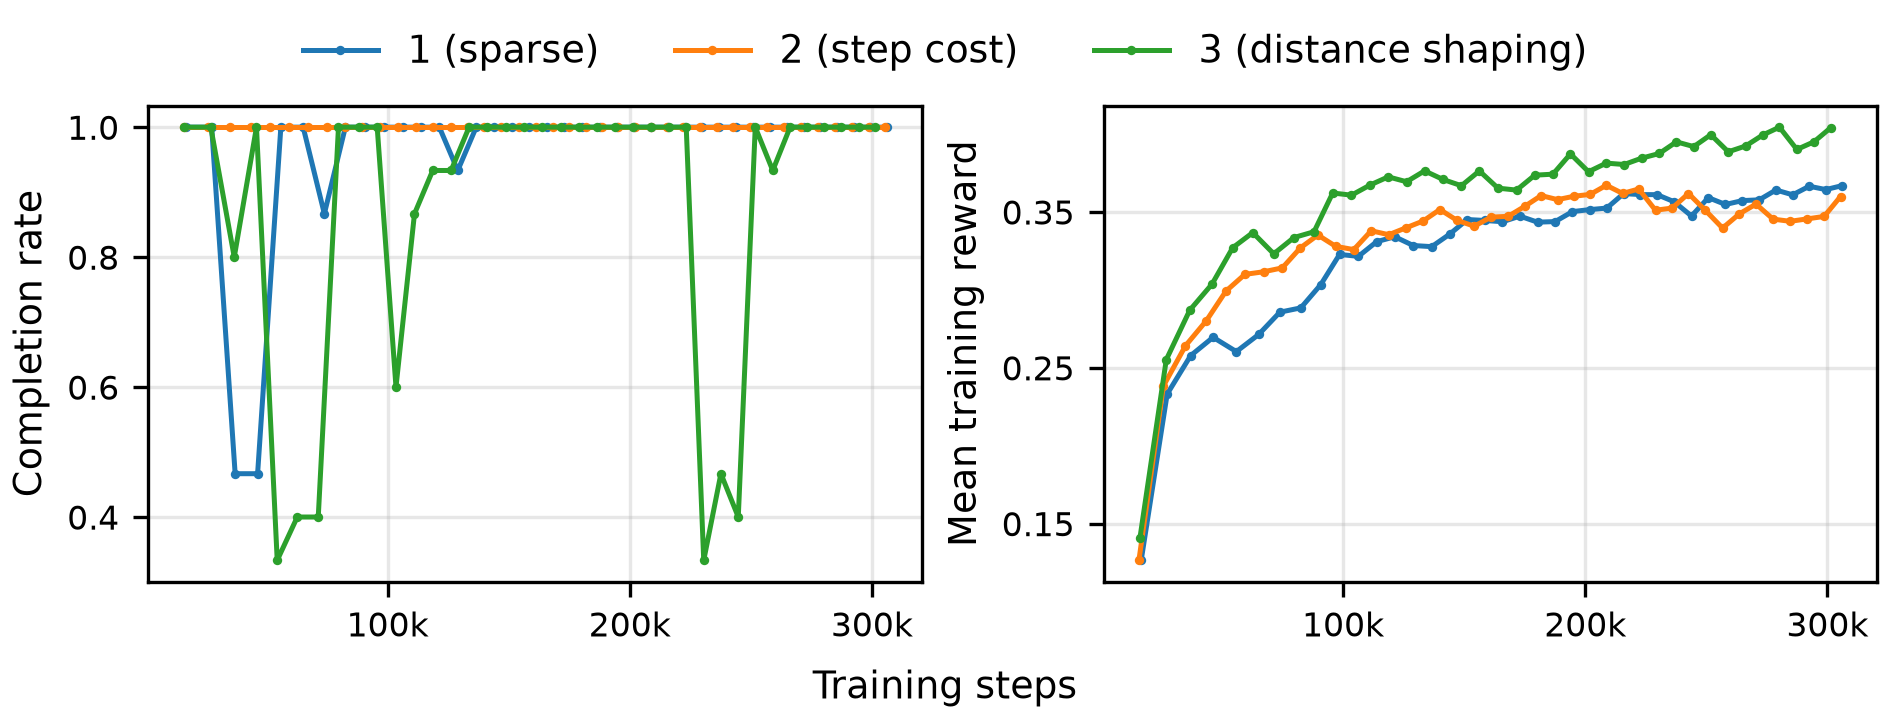
\includegraphics[width=0.85\textwidth]{task1_reward_comparison.png}
		\caption{Evaluation bursts (15 games each) of the three reward configurations during training.}
		\label{fig:rhine_stage_a_comparison}
	\end{figure}
	
	The evaluation bursts during training discriminate better (Figure~\ref{fig:rhine_stage_a_comparison}). Configuration 3 has the highest raw training reward only because the shaping term inflates it. It was the least stable configuration: 12 of 38 evaluation points fell below full completion and 6 below 0.5, including a regression to 0.33 late in training, and the last ten points averaged only 0.88. Configuration 1 dropped below 0.5 twice, both early in training. Configuration 2 never fell below full completion in 41 evaluation points and was selected. The discarded distance shaping is not rejected in general. On this dense board, the step cost alone already supplies enough pressure towards efficiency.
	
	
	\paragraph{Zero-shot transfer to \texttt{coin-heaven-9}.} The completion rate transfers without loss (Table~\ref{tab:rhine_task1_zero_shot}). Steps per coin roughly double, but this is structural: with fewer coins on the same board, the distance between successive coins is larger for any policy. The wait fraction stays at zero, no illegal actions occur outside the training scenario, and the step counts are tightly clustered across the 100 maps, so the conditional fine-tuning stage was not run.
	
	\begin{table}[htbp]
		\centering
		\begin{tabular}{lcc}
			\toprule
			Metric & \texttt{coin-heaven} & \texttt{coin-heaven-9}, zero-shot \\
			\midrule
			Completion rate & 1.00 & 1.00 \\
			Steps to completion (mean / s.d.) & 125.17 / 10.26 & 49.15 / 7.39 \\
			Steps per coin & 2.503 & 5.461 \\
			Wait fraction & 0.0005 & 0.000 \\
			Illegal actions & 0 & 0 \\
			\bottomrule
		\end{tabular}
		\caption{Zero-shot transfer of the selected configuration (Configuration 2), 100 games each.}
		\label{tab:rhine_task1_zero_shot}
	\end{table}
	
	
	\section{Task 2 Results}
	\label{subsec:rhine_results_task2}
	
	\paragraph{Shaping becomes necessary.} Unlike in Task 1, target-progress shaping was decisive on the crate board. Without it the agent collapsed into waiting (wait fraction about 0.88, about 14 crates destroyed, no completed games), whereas the shaped agent rarely waited and destroyed 88 to 93 crates per game. The shaped reward became the baseline for all later work.
	
	\paragraph{Oscillation and its remedies.} The shaped agent then oscillated between a bombing position and an adjacent tile. The shaping gives no net reward for such a loop, and BOMB remained legal throughout, so the mask was not the cause. Table~\ref{tab:rhine_task2_ablation} compares the reward changes tested against it. A penalty that counted only steps on a bombing tile never triggered, because the loop left that tile every other step. Adding reward for crates destroyed when no coin was reachable removed oscillation only by replacing it with a complete freeze. A penalty based on the last four positions did not reduce oscillation but greatly improved crate clearing and was adopted. 
	
	\begin{table}[htbp]
		\centering
		\small
		\begin{tabular}{lccccc}
			\toprule
			Configuration & Oscillation & Crates & Wait & Completion & Adopted \\
			\midrule
			Shaped reward (baseline) & 0.133 & 59.2 & 0.475 & 0.00 & -- \\
			+ penalty on bombing-tile steps & 0.500 & 49.8 & 0.460 & 0.03 & $\times$ \\
			+ crate reward without reachable coin & 0.000 & 15.2 & 0.881 & 0.03 & $\times$ \\
			+ penalty on last four positions & 0.133 & 118.0 & 0.037 & 0.33 & $\checkmark$ \\
			\bottomrule
		\end{tabular}
		\caption{Reward changes against oscillation on \texttt{loot-crate} (single seed, 30 games, unequal training lengths).}
		\label{tab:rhine_task2_ablation}
	\end{table}
	A feature encoding the agent's recent positions was later tested on two seeds of the final configuration described below. On the same seeds it lowered oscillation from 0.155 to 0.070, but completion was unchanged and the difference lay within the spread between seeds, so it was not adopted. Without such a history, the feature vector was identical at every visit to the same tile, so the policy cannot condition on how long it has been stuck, and reward penalties alone cannot stop the loop. This motivated the evaluation-time breaker (Section~\ref{subsec:rhine_mask}). With the breaker enabled during evaluation, the number of oscillating games fell from 11/300 to 0/300 and the completion rate rose from 0.823 to 0.847.
	
	\paragraph{Training instability.} Throughout Task 2, the periodic evaluations alternated between good phases and collapses in which few crates were destroyed, and none of the later runs, including all runs of the final configuration, reached a stable level before its step limit. Two changes were kept. Return normalization kept the value loss between 0.26 and 0.37 instead of growing to 4.55 and made the collapses shorter, but the alternation remained. A rollout length of 4096 instead of 2048 steps gave, in a single seed, the best final result among these unstable runs and was therefore kept, although it did not remove the alternation either. Entropy and learning-rate decay did not resolve the collapses, an entropy coefficient of 0.05 gave opposite outcomes on two seeds, $\lambda = 0.90$ in GAE was worse than $0.95$ for both seeds, and a larger separate critic left the explained variance at 0.03--0.15. None of these was adopted.
	
	\paragraph{Bombing-target selection.} The bombing target was initially the nearest reachable bombing tile, so the agent often ignored a slightly farther tile where a bomb would destroy many more crates. Two changes to this choice were tested. Safety was already guaranteed by the action mask, which allows BOMB only when an escape route exists (Section~\ref{subsec:rhine_mask}). The target could, however, be a tile on which the mask never allowed BOMB, and such targets caused the freeze described above. A safety filter therefore kept only candidate tiles with an escape route. Crate-target scoring instead chooses the tile that maximizes $c/(d+1)$ (Section~\ref{subsec:rhine_features}), accepting a few extra steps for more crates per bomb. In a two-by-two comparison (Table~\ref{tab:rhine_task2_targets}), scoring alone gave the best results, with more crates destroyed, a higher completion rate and less oscillation than the baseline. The filter raised oscillation whether used alone or together with scoring and cancelled most of the scoring's gain in completion, while the self-kill rate was zero in all runs with or without it. The final configuration therefore uses scoring without the filter.
	
	\begin{table}[htbp]
		\centering
		\small
		\begin{tabular}{lcccc}
			\toprule
			Configuration & Crates & Wait & Completion & Oscillation \\
			\midrule
			Baseline (5 seeds) & 71.0 & 0.333 & 0.126 & 0.316 \\
			+ safety filter & 97.4 & 0.057 & 0.140 & 0.570 \\
			+ crate-target scoring & 117.0 & 0.063 & 0.585 & 0.155 \\
			+ both & 100.4 & 0.108 & 0.240 & 0.575 \\
			\bottomrule
		\end{tabular}
		\caption{Bombing-target selection on \texttt{loot-crate} (two seeds per variant, about 500k training steps, 100 evaluation games).}
		\label{tab:rhine_task2_targets}
	\end{table}
	
	\paragraph{Final Task 2 agent.} On \texttt{classic}, without further training, the final agent completed 99\% of games, destroyed 123.1 crates on average, waited in 4.5\% of steps, and had no self-kills or oscillating games. A second evaluation seed gave the same completion rate. The fine-tuning stage on \texttt{classic} was therefore not needed.
	
	\section{Task 3 Results}
	\label{subsec:rhine_results_task3}
	
	Table~\ref{tab:rhine_task3} summarizes the four stages. Scores are not comparable across stages, because the number and type of opponents determine how many kills are possible. Navigation and crate clearing were retained throughout, with completion rates of at least 0.87.
	
	\begin{table}[H]
		\centering
		\small
		\resizebox{\textwidth}{!}{%
			\begin{tabular}{llcccccc}
				\toprule
				Stage & Opponents & Score & Kills & Self-kill & Killed by opp. & Completion & Oscillation \\
				\midrule
				A & 1 peaceful & 12.39$\pm$0.11 & 0.77$\pm$0.03 & 0.000$\pm$0.000 & 0.000 & 0.88$\pm$0.06 & 0.043$\pm$0.021 \\
				B & 3 peaceful & 19.05$\pm$1.00 & 2.11$\pm$0.18 & 0.003$\pm$0.006 & 0.000 & 0.87$\pm$0.06 & 0.030$\pm$0.010 \\
				C & 1 coin collector & 6.11$\pm$0.49 & 0.08$\pm$0.05 & 0.053$\pm$0.015 & 0.000 & 0.99$\pm$0.01 & 0.010$\pm$0.017 \\
				D & 3 coin collectors & 4.58$\pm$0.40 & 0.40$\pm$0.05 & 0.063$\pm$0.012 & 0.017$\pm$0.006 & 1.00$\pm$0.00 & 0.007$\pm$0.006 \\
				\bottomrule
			\end{tabular}%
		}
		\caption{Task 3 results.}
		\label{tab:rhine_task3}
	\end{table}
	
	\paragraph{Escape routes and opponents.} Against the coin collector, all 16 self-kills recorded before the fix followed the same pattern. An escape route that was valid when the bomb was placed was later blocked by an opponent moving along it, often at the second or third step rather than the first. Rewriting the escape check to test every tile of the route (Section~\ref{subsec:rhine_mask}) eliminated this pattern: none recurred after retraining. About 90\% of the remaining self-kills (26/29 in an earlier Stage C version, 17/19 in Stage D) occur when the agent and an opponent try to enter the same tile in the same step. The framework resolves this in random order and reports the loser's move as invalid. Because this is decided after the action is submitted, neither the mask nor training can change its outcome, and its share did not change when the number of opponents rose from one to three.
	
	\paragraph{Learning to attack.} In Stage C, the agent rarely bombed when an opponent was in range, and the policy's bombing probability was almost uncorrelated with the kill-target features (correlations between $-0.03$ and $0.14$ across seeds). Changing the aggregation of the escape-difficulty score from a sum to a maximum did not change this. First-layer weight norms showed that the network amplified the crate-count feature about four times relative to its random initialization, but the kill-value feature only about 1.1 times. This was attributed to kill rewards being too rare against a single opponent for the value of attacking to be learned. With three opponents in Stage D, kill opportunities became frequent and the agent took 66\% of them, but only 1.6\% of those bombs killed. The agent had learned to attack but not to aim.
	
	\paragraph{Mask variants.} Two stricter masks were evaluated offline on the Stage D games: requiring an additional step of margin against opponents on escape routes, and forbidding bombs while in danger whenever a safe alternative exists. The first would have prevented at most 5 of 17 same-tile self-kills, but would also have blocked 9.5\% of all bombs, 89\% of which covered an opponent. Both variants were rejected because their cost in attack opportunities outweighed the small number of deaths they could avoid.
	
	\paragraph{Oscillation breaker.} In a separate evaluation of the Stage B checkpoints, disabling the breaker raised the oscillation fraction from 0.013 to 0.487 and lowered the score from 18.9 to 17.7. In Stage D it lowered oscillation from 0.267 to 0.007, while the score difference stayed within noise.
	
	\paragraph{Zero-shot transfer to the rule-based agent.} Evaluated against three \texttt{rule\_based\_agent}s without further training, the Stage D agent scored 5.00$\pm$0.54. Its self-kill rate rose from 0.063 against its training opponents to 0.153$\pm$0.104, and its killed-by-opponent rate from 0.017 to 0.107$\pm$0.006. This evaluation serves as the baseline in Task 4.
	
	\section{Task 4 Results}
	\label{subsec:rhine_results_task4}
	
	\paragraph{Final evaluation and controlled baseline.} Under identical evaluation settings, the Task 4 agent scored 6.33 against 5.00 for the Stage D agent (Table~\ref{tab:rhine_task4}), a difference of $+1.33$ with a standard error of 0.30 over 300 games. The gain came from more kills (0.58 instead of 0.34 per game), while the self-kill and killed-by-opponent rates changed by 0.04 or less, neither significantly.
	
	\begin{table}[H]
		\centering
		\small
		\begin{tabular}{lccccc}
			\toprule
			Agent & Score & Kills & Self-kill & Killed by opp. & Oscillation \\
			\midrule
			Stage D agent (baseline) & 5.00$\pm$0.54 & 0.34$\pm$0.07 & 0.153$\pm$0.104 & 0.107$\pm$0.006 & 0.007$\pm$0.012 \\
			Task 4 agent, breaker on & 6.33$\pm$0.76 & 0.58$\pm$0.19 & 0.113$\pm$0.025 & 0.130$\pm$0.026 & 0.007$\pm$0.006 \\
			Task 4 agent, breaker off & 6.27$\pm$1.28 & 0.58$\pm$0.27 & 0.140$\pm$0.050 & 0.097$\pm$0.023 & 0.250$\pm$0.066 \\
			\bottomrule
		\end{tabular}
		\caption{Task 4 evaluation against three \texttt{rule\_based\_agent}s.}
		\label{tab:rhine_task4}
	\end{table}
	
	\paragraph{Comparison with the rule-based agent.} Figure~\ref{fig:rhine_vs_rulebased} compares RHINE with its three opponents in the same games. RHINE averaged 6.33 points, more than the best of the three opponents in each game (5.04), and finished alone in first place in 53\% of games (63\% including ties). The untrained Stage D agent scored 5.00 against 5.22 for the best opponent and finished alone in first place in 41\% of games. Under the second evaluation seed, the Task 4 agent scored 6.11 against 4.84 and finished alone in first place in 52\% of games.
	
	\begin{figure}[htbp]
		\centering
		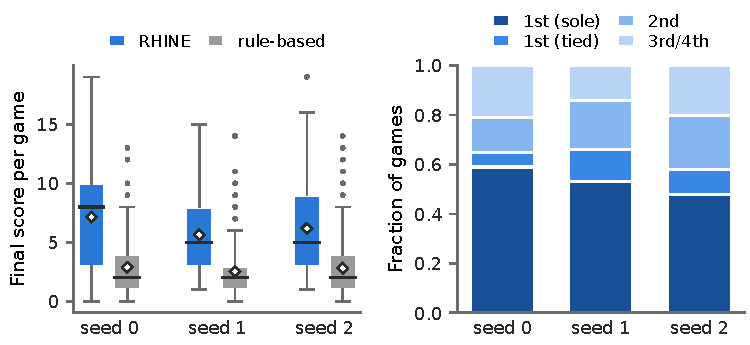
\includegraphics[width=0.7\textwidth]{task4_vs_rule_based.pdf}
		\caption{Per-game final scores of RHINE and its opponents (left, diamonds mark the mean) and RHINE's placement among the four agents (right).}
		\label{fig:rhine_vs_rulebased}
	\end{figure}
	
	\paragraph{Oscillation breaker and deadlock bombing.} As in Stage D, the breaker removed oscillation without changing the score or measurably changing the death rates (Table~\ref{tab:rhine_task4}). A further evaluation-only rule forced a bomb when the agent was confined as defined for the breaker, no crates or coins remained, its current tile's blast covered an opponent, and BOMB was legal under the mask. It fired on 72 steps in 300 games, but changed the chosen action on only 28 of them, because the policy had already chosen BOMB on the others. It produced no significant gain (6.40 versus 6.33) and was not adopted.
	
	
	\paragraph{Where the remaining deaths come from.} Of the 73 deaths in the final configuration (34 self-kills and 39 kills by opponents), 50 (68\%) resulted from losing a same-step contest for a tile the agent needed to escape, shortly before death. This covers 30 of the self-kills and 20 of the deaths caused by opponents, and as in Task 3 it cannot be prevented by the mask. One of these contests repeats exactly: after bombing near the corner tile (15,1), seed 0 flees into the dead end towards the corner instead of the open side and loses the contest for its only exit, with the same sequence of actions in 6 of 100 games. The Stage D agent of seed 1 dies there in the same way in 15 of 100 games, so the pattern is tied to the corner's geometry rather than to one checkpoint. In 16 further deaths caused by opponents, the agent was trapped without a contest: in 13 an opponent's body blocked its escape route, and in 3 blast danger closed a dead end. In all 16 the mask left only WAIT for the last two to five steps before a single opponent's bomb killed the agent. The number of free tiles reachable within six steps narrowed at least four steps before 94.9\% of the deaths caused by opponents and 38.2\% of the self-kills, but also at 27.7\% of randomly chosen moments that were not followed by death, so this feature alone is too unspecific to trigger an intervention.
	
	\paragraph{Attacking.} In 3222 of 6270 opportunities (51\%) the agent placed a bomb that covered an opponent's current tile, and 4.7\% of those bombs killed. When a covered opponent, judged from the current positions, had no safe path out of the blast and BOMB was legal, the agent bombed in 87\% of these steps, and 44\% of these bombs killed within five steps. The limiting factor is therefore creating situations in which an opponent is trapped, not the willingness to attack when one arises.
	
	\paragraph{Final agent.} The submitted agent is the seed-0 checkpoint of Task 4 with the oscillation breaker enabled, which scored highest under both evaluation seeds (Table~\ref{tab:rhine_task4_seeds}). Under both evaluation seeds, the scores of the three seeds follow their kill rates. Seed 0 also has the highest self-kill rate, so the differences between seeds come from attacking rather than from survival.
	
	\begin{table}[htbp]
		\centering
		\small
		\begin{tabular}{lcccc}
			\toprule
			Training seed & Score & Kills & Self-kill & Killed by opp. \\
			\midrule
			0 & 7.15 / 7.48 & 0.78 / 0.87 & 0.14 / 0.17 & 0.14 / 0.12 \\
			1 & 5.64 / 5.17 & 0.40 / 0.35 & 0.11 / 0.07 & 0.10 / 0.17 \\
			2 & 6.20 / 5.67 & 0.57 / 0.50 & 0.09 / 0.08 & 0.15 / 0.21 \\
			\bottomrule
		\end{tabular}
		\caption{Task 4 agent per training seed, under evaluation seed 1000 / 2000.}
		\label{tab:rhine_task4_seeds}
	\end{table}
	
	% ================================================================
	% 7. CONCLUSION
	% ================================================================
	
	\chapter{Conclusion}
	\label{chap:conclusion}
	\label{sec:rhine_conclusion}
	
	\section{Findings} A small PPO agent on engineered features, with a rule-based safety mask, learned each task from scratch and in the end beat three \texttt{rule\_based\_agent}s: it finished first alone in more than half of the games and averaged 6.3 points against 5.0 for the strongest opponent in each game. Reward shaping behaved differently depending on reward density. It destabilized learning on the dense coin board but was indispensable once crates made rewards sparse. Oscillation proved to be a limitation of the Markovian state rather than of the reward, and the evaluation-time breaker removed it at no cost in score, although it is a rule, not a learned skill. The Task 4 agent scored significantly higher than the Stage D agent without measurably fewer deaths. Most remaining deaths come from same-step tile contests that the agent cannot control. The score differs between training seeds by more than it differs between the Task 4 agent and the Stage D agent.
	
	\section{Improvements with more time}
	\begin{itemize}[noitemsep]
		\item \textbf{Attack training.} The score follows the kill rate, and the agent already bombs trapped opponents in most cases, so training should reward creating traps rather than raise the kill reward.
		\item \textbf{Seed dependence.} More training seeds, with selection or ensembling across them, would make the final agent less dependent on a single run.
		\item \textbf{Escape planning.} Most deaths caused by opponents without a contest occurred after an opponent's body blocked the escape route. Escape planning that anticipates opponents' next moves could address these and the repeated death at one corner tile.
		\item \textbf{Oscillation.} A learned memory of recent positions, for example stacked frames or a recurrent layer, could address oscillation within the policy instead of through a rule, since a hand-crafted position-history feature gave no clear gain. The confinement penalty, adopted in Task 2 before the breaker existed, was never re-evaluated. Retraining without it would show whether it still contributes.
		\item \textbf{Opponent diversity.} Training against mixed opponents or against earlier versions of the agent itself would test whether the agent can judge an unlabelled opponent's threat from its behaviour.
	\end{itemize}
	
	\section{Suggestions for the game setup}
	\begin{itemize}[noitemsep]
		\item \textbf{Tile contests.} When two agents move onto the same tile, the loser is determined by a random processing order and its move is lost. This was the largest single cause of RHINE's deaths, and the agent cannot influence its outcome. Letting agents submit several actions ranked by preference, with the next one executed when the first fails, would make such contests a matter of design rather than chance.
		\item \textbf{Reproducibility.} The provided \texttt{rule\_based\_agent} and \texttt{coin\_collector\_agent} reseed their random number generators from system entropy, so evaluations with a fixed seed are not reproducible without patching them.
		\item \textbf{Thinking-time limit.} The limit is measured in wall-clock time, so pauses of the host machine count against the agent, and it is not documented which parts of the framework's own processing fall within the limit.
		\item \textbf{Working directory.} During callbacks the framework changes the working directory to the agent's folder, which silently breaks relative file paths used in training code.
	\end{itemize}
	
	
	\begin{thebibliography}{9}
		\bibitem{bengio2009curriculum} Y.~Bengio, J.~Louradour, R.~Collobert, and J.~Weston. Curriculum learning. In \emph{Proceedings of the 26th International Conference on Machine Learning (ICML)}, 2009.
		\bibitem{henderson2018matters} P.~Henderson, R.~Islam, P.~Bachman, J.~Pineau, D.~Precup, and D.~Meger. Deep reinforcement learning that matters. In \emph{Proceedings of the AAAI Conference on Artificial Intelligence}, 2018.
		\bibitem{huang2022masking} S.~Huang and S.~Onta\~{n}\'{o}n. A closer look at invalid action masking in policy gradient algorithms. In \emph{Proceedings of the 35th International FLAIRS Conference}, 2022.
		\bibitem{ng1999shaping} A.~Y. Ng, D.~Harada, and S.~Russell. Policy invariance under reward transformations: Theory and application to reward shaping. In \emph{Proceedings of the 16th International Conference on Machine Learning (ICML)}, 1999.
		\bibitem{schulman2016gae} J.~Schulman, P.~Moritz, S.~Levine, M.~I. Jordan, and P.~Abbeel. High-dimensional continuous control using generalized advantage estimation. In \emph{International Conference on Learning Representations (ICLR)}, 2016.
		\bibitem{schulman2017ppo} J.~Schulman, F.~Wolski, P.~Dhariwal, A.~Radford, and O.~Klimov. Proximal policy optimization algorithms. \emph{arXiv preprint arXiv:1707.06347}, 2017.
	\end{thebibliography}
\end{document}